\documentclass[11pt]{article}
\usepackage{graphicx} % This lets you include figures
\usepackage{hyperref} % This lets you make links to web locations
\usepackage[margin=0.5in]{geometry}
\usepackage[rightcaption]{sidecap}
\usepackage{subcaption}
\usepackage{wrapfig}
\usepackage{float}
\usepackage{imakeidx}
\usepackage{indentfirst}
\makeindex
%---------------------------Do Not Edit Anything Above This Line!!------------------------

% edit the line below, if needed, to change the directory name for your image files.
\graphicspath{ {./images/} }



\begin{document}

%---------------------------Edit Content in the Box to Create the Title Page--------------
\begin{titlepage}
   \begin{center}
       \vspace*{1cm}
	   \Huge
       \textbf{GPS Based Campus Room Finder}

       \vspace{0.5cm}
       \Large
       Sprint 3 \\
       10/27/2025 \\
   \end{center}

       \vspace{1.5cm}

\begin{table}[h!]
\centering
\begin{tabular}{|l|l|}
\hline
\textbf{Name} & \textbf{Email Address} \\ \hline
Aaron Downing         & aaron.downing652@topper.wku.edu         \\ \hline
Ryerson Brower         & ryerson.brower178@topper.wku.edu         \\ \hline
Kaden Hunt         &  kaden.hunt144@topper.wku.edu         \\ \hline
\end{tabular}
\end{table}

%Latex Table Generator    
%https://www.tablesgenerator.com/     
        
\vspace{4in}

\centering        
Client: Michael Galloway \\
CS 360 \\
Fall 2025\\
Project Organization Documentation

\end{titlepage}
%---------------------------Edit Content in the Box to Create the Title Page--------------


% No text here.


%---------------------------Do Not Edit Anything In This Box!!------------------------
%Table of contents and list of figures will be autogenerated by this section.
\newpage
\setcounter{page}{1}%
\cleardoublepage
\pagenumbering{gobble}
\tableofcontents
\cleardoublepage
\pagenumbering{arabic}
\clearpage
\newpage
\setcounter{page}{1}%
\cleardoublepage
\pagenumbering{gobble}
\listoffigures
\cleardoublepage
\pagenumbering{arabic}
\newpage
%---------------------------Do Not Edit Anything In This Box!!------------------------

% No text here.


%---------------------------Project Team's Organizational Approach------------------------------
\section{Project Team's Organizational Approach} %\section{} is used to create major section headers
%100 words for each sprint
    %How/where did the group meet?  How often did you meet as an entire team?  Who’s the Project Manager for this sprint?
	Sprint 1: Kaden Hunt served as the Project Manager for this sprint. The entire team met in person once per week for hour-long working sessions at the Commons on Thursdays at 2:00 PM. To maintain continuous collaboration, the group utilized a Discord server for ongoing chat, video calls, and file sharing, along with text messaging for quick updates. Furthermore, the team held brief, 20-minute meetings with the client every Tuesday to present a prepared progress report, ensuring alignment and feedback on our development process. 
    
	%How/where did the group meet?  How often did you meet as an entire team?  Who’s the Project Manager for this sprint?
	Sprint 2: For this sprint, the team maintained the same overall meeting structure, continuing to gather weekly in person at the Commons on Thursdays at 2:00 PM. These meetings were used to coordinate progress, divide work, and review draft materials together. The client meetings on Tuesdays also continued, providing regular opportunities for feedback. The primary focus of Sprint 2 shifted toward software modeling and design. Team members were responsible for producing UML diagrams and design pattern documentation, which were reviewed collectively during meetings to ensure consistency. This sprint emphasized collaboration around visual modeling, so the group spent more time walking through diagrams together, making sure the representations were aligned with the project. Project Manager Ryerson Brower ensured the task list was up to date and that contributions were balanced across members, while texting was used to coordinate outside of scheduled times.
 
    
    %How/where did the group meet?  How often did you meet as an entire team?  Who’s the Project Manager for this sprint?
	Sprint 3: For this sprint, the team maintained the same overall meeting structure, continuing to gather weekly in person at the Commons on Thursdays at 2:00 PM. These meetings were used to coordinate progress, divide work, and review draft materials together. The client meetings on Tuesdays also continued, providing regular opportunities for feedback. The primary focus of Sprint 3 progress visibility centered on the development of wire-frames and storyboards, along with addressing different security risks, and with getting close to a final product by making our app UI. Team members were responsible for producing wireframes, s, and researching security risks. Which were reviewed collectively during meetings to ensure consistency. Project Manager Ryerson Brower ensured the task list was up to date and that contributions were balanced across members, while texting was used to coordinate outside of scheduled times.

    %How/where did the group meet?  How often did you meet as an entire team?  Who’s the Project Manager for this sprint?
	Sprint 4: 



%---------------------------End Project Team's Organizational Approach------------------------------


% No text here.


%---------------------------Schedule Organization---------------------------------------------------
\section{Schedule Organization}
%Gantt charts cover the tasks/time commitments and estimations for the entire project.  We will have four iterations of the Gantt Chart, with iteration focusing on a specific sprint.

\subsection{Gantt Chart v1:}
%100 words to describe the focus for this sprint.
%Identify the location for the Gantt Chart created during Sprint 1.  Should be clearly labeled in the project directory.

The focus for Sprint 1 was focused on project initiation, team formation, and foundational planning. The primary tasks involved establishing team roles and responsibilities, setting up collaboration tools like GitHub and Google Docs, and drafting the initial versions of both the Organizational and Technical documentation. This chart outlined the critical path for researching project requirements, defining the scope, and performing an initial risk analysis to ensure the project's viability. The chart is located in the project directory at: TopperNav/docs/TopperNav\_Gantt\_Chart\_Sprint2.png



\subsection{Gantt Chart v2:}
%100 words to describe the focus for this sprint.
%Identify the location for the Gantt Chart created during Sprint 2.  Should be clearly labeled in the project directory.
The focus for Sprint 2 was on software modeling and design. Tasks included creating UML diagrams such as use case, sequence, state, component, and deployment diagrams, as well as developing class diagrams tied to design patterns. Additional deliverables included defining system boundaries, producing an updated risk analysis, and a requirements tracability table. The team also worked on both technical and organizational documentation and preparing the Sprint 2 presentation. This sprint represented the transition from planning into detailed design, with a emphasis on visual artifacts that demonstrate how the system will operate. The Gantt chart for Sprint 2, outlining these milestones and due dates, is located in the project directory at: TopperNav/docs/TopperNav\_Gantt\_Chart\_Sprint2.png




\subsection{Gantt Chart v3:}
%100 words to describe the focus for this sprint.
%Identify the location for the Gantt Chart created during Sprint 3.  Should be clearly labeled in the project directory.
The focus for Sprint 3 was on software implementation and design. Tasks included, wireframes/storyboards, user experience, product security, product performance. Additional deliverable included defining system boundaries defining different security requirements and techniques, here we also needed to start getting test results. But our group took a different approach, we wanted to get our UI for the app done first. So at the moment we don't have much for us to test but we got a visual product and a UI. The team also worked on both technical and organizational documentation and preparing the Sprint 3 presentation. This sprint represented the transition from planning into actual implementation of the and getting close to the final product.
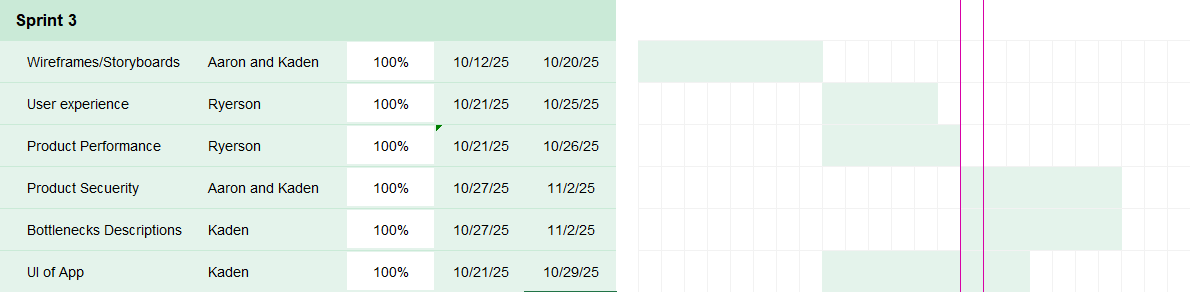
\includegraphics[scale=0.7]{images/gantt chart 3.png} 


\subsection{Final Gantt Chart:}
%100 words to describe the focus for this sprint.
%Identify the location for the Gantt Chart created during Sprint 4.  Should be clearly labeled in the project directory.



%---------------------------End Schedule Organization---------------------------------------------------


% No text here.


%---------------------------Progress Visibility---------------------------------------------------
\section{Progress Visibility}
%100 words for each sprint.
%For each sprint, explain how each member of the group is progressing with assigned tasks and how that progress is shared with the group.  Also, explain how the group is progressing with assigned tasks and how that progress is shared with the client.  Examples:  how does the group assign tasks?  How to group members know tasks assigned to them?  How do group members communicate when assigned tasks are complete, need assistance, or waiting on other tasks to be completed first?
\subsection{Sprint 1 Progress Visibility}

The team progressed steadily through Sprint 1 and completed the deliverables before the due date. Tasks were divided among members during class and reinforced during weekly meetings. Kaden Hunt managed the task list, prepared the presentation, and contributed to both the Organizational and Technical documentation. Aaron created the Gantt chart and also worked on sections of both documents, while Ryerson focused on contributing to the documentation. Progress visibility within the group was maintained through frequent conversations, updates in the group chat and Discord, and use of the GitHub Projects page. The Gantt chart also provided a clear overview of tasks and deadlines, ensuring accountability. Through these resources, members could report when tasks were complete, request assistance, or flag dependencies. Overall, consistent communication and shared tools allowed the team to remain coordinated and deliver Sprint 1 successfully.


\subsection{Sprint 2 Progress Visibility}
During Sprint 2, progress visibility centered on the development of diagrams and design materials. Tasks were assigned during meetings and tracked via texts or the next in person meeting. Team members communicated their progress through texts as well, posting drafts of diagrams for feedback before finalizing them. The use of visual diagrams required collaborative review, so much of the work was shared early and discussed during weekly meetings. Updates to documentation and the presentation slides were also reviewed as a group to ensure consistency across deliverables. Progress for the client was summarized in the weekly report and presented at Tuesday meetings, which gave the team an opportunity to confirm the project was on track before moving forward. This cycle of assignment, discussion, and review allowed the group to stay on schedule and adapt when tasks needed additional attention.


\subsection{Sprint 3 Progress Visibility}
During Sprint 3, progress visibility centered on the development of wire-frames and storyboards, along with addressing different security risks, and with getting close to a final product by making our app UI. Tasks were assigned during meetings and tracked via texts or the next in person meeting. Team members communicated their progress through texts as well, posting drafts of diagrams for feedback before finalizing them. The use of visual diagrams required collaborative review, so much of the work was shared early and discussed during weekly meetings. Updates to documentation and the presentation slides were also reviewed as a group to ensure consistency across deliverables. Progress for the client was summarized in the weekly report and presented at Tuesday meetings, which gave the team an opportunity to confirm the project was on track before moving forward. This cycle of assignment, discussion, and review allowed the group to stay on schedule and adapt when tasks needed additional attention.

\subsection{Sprint 4 Progress Visibility}
Text goes here.

%---------------------------End Progress Visibility---------------------------------------------------

% No text here.


%---------------------------Software Process Model---------------------------------------------------
\section{Software Process Model}
%150 words
%Describe in this section the Software Process Model used and how it increases the quality of the final deliverables.  The team should also define the quality control steps that are used in the Software Process Model.

Our team adopted the Iterative Software Process Model, which emphasizes building the project in small, repeatable cycles. This approach allowed us to steadily refine our work by dividing development into manageable stages and reviewing progress continuously. Unlike a linear model, the iterative approach gave us the flexibility to adjust plans based on what we learned along the way, which helps reduce risk and increases the quality of the final deliverables.

During Sprint 1, our focus was on preparation and foundational work. Quality control steps included producing clear documentation, researching relevant tools and requirements, and delivering a presentation to communicate progress. We also treated environment setup as part of quality assurance by ensuring all team members had the same software installed, including Android Studio, the JDK, TeX Live, and TeXmaker. These checks provided consistency across the team and created a strong base for future development cycles.

Dor Sprint 2, our team continued with the Iterative Software Process Model, focusing on refinement and incremental progress. Each cycle allowed us to revisit earlier work while introducing new features, ensuring flexibility and adaptability. This helped us incorporate feedback from Sprint 1 and quickly adjust designs or diagrams as our understanding of the project matured.

In this sprint, we placed stronger emphasis on design artifacts and system modeling, including UML diagrams (use case, sequence, state, component, and deployment). These served as both technical blueprints and quality checks, ensuring requirements were being met. Quality assurance also included maintaining consistency across diagrams through member check ins.By combining documentation updates with incremental design work, Sprint 2 advanced the project from planning into concrete models, providing a clearer roadmap for coding in later sprints.

%---------------------------End Software Process Model---------------------------------------------------

% No text here.


%---------------------------Risk Management--------------------------------------------------------------
\section{Risk Management}
%Use this section to describe the team's approach to risk management.

\subsection{Risk Identification}
%List, categorize, and prioritize all potential risks associated with the project.
The following risks are listed and categorized by potential risk level.

\begin{itemize}
    \item \textbf{Database Performance (High Priority):} The database may become too slow under heavy loads, affecting responsiveness and user experience.
    \item \textbf{Route Generation API Failure (High Priority):} The external route generation API may not function as expected, preventing key functionality of the application.
    \item \textbf{Compatibility Issues (Medium Priority):} The system may encounter compatibility problems across different devices, operating systems, or software versions.
    \item \textbf{Access to Android Phones (Medium Priority):} Limited availability of Android devices for testing may hinder progress.
    \item \textbf{Large File Download (Low Priority):} Users may face issues when downloading or uploading large files, leading to performance bottlenecks.
\end{itemize}

\subsection{Risk Planning}
%Give overviews of plans for specific risk types
The team has outlined the following plans for risk planning:

\begin{itemize}
     \item \textbf{Database Performance:} Implement query optimization, proper indexing, and caching strategies. Load testing will be performed early to identify bottlenecks.
    \item \textbf{Route Generation API Failure:} Identify and test backup APIs during early development. 
    \item \textbf{Compatibility Issues:} Use emulators and virtual machines to ensure broader compatibility across various platforms.
    \item \textbf{Access to Android Phones:} Gain access to an android phone temporarily and share them among team members as needed. 
    \item \textbf{Large File Download:} Implement file compression. Clearly communicate file size limitations to users.
\end{itemize}

\subsection{Risk Monitoring}
%Give overviews of how the team will monitor specific types of risks
The following monitoring strategies will be used for the remaining duration of the project:

\begin{itemize}
    \item \textbf{Database Performance:} Monitor query execution times and system performance.
    \item \textbf{Route Generation API Failure:} Implement automated alerts for API failures or unusual latency.
    \item \textbf{Compatibility Issues:} Maintain a compatibility checklist and update it with each system change.
    \item \textbf{Access to Android Phones:} Track device usage and availability within the team. .
    \item \textbf{Large File Download:} Monitor client feedback related to file transfers.
\end{itemize}


%---------------------------Risk Management--------------------------------------------------------------





%example image:  uncomment to show usage
%\begin{figure}[h]
%    \centering
%    \includegraphics[width=1\textwidth]{images/Add_non-music.png}
%    \caption{This is how you add non-music items.}
%    \label{fig16}
%\end{figure}


%example links:  uncomment to show usage.
%\url{https://www.youtube.com}
%\href{https://www.wku.edu/}{WKU Homepage}
%\footnote{You can put the link in a footnote like this.}

% Anything to the right of a percent sign will be ignored by LaTeX.
% You can use this to put notes to yourself.  



\end{document}
